\documentclass{article}
\usepackage{amsmath, amsthm, amssymb}
\usepackage{listings}
\usepackage{graphicx}
\usepackage{float}
\usepackage{enumerate}
\usepackage{fancyhdr, lastpage,booktabs}
\usepackage{polynom}
\usepackage[left=0.75in, top=1.00in, right=0.75in, bottom=1.00in]{geometry}

\usepackage{graphicx}
\usepackage{tikz}
\usetikzlibrary{backgrounds}
\usepackage{amssymb}

\tikzstyle{cover}=[rectangle,inner sep=1pt,outer sep=0pt]
\tikzstyle{nb}=[fill=red]
\tikzstyle{lv}=[fill=black!80]
\tikzstyle{bd}=[fill=black]

\usepackage{wrapfig}
\usepackage{lmodern}
\usepackage{blindtext}

\usepackage{float}
\restylefloat{figure}

\pagestyle{fancy}
\setlength{\headheight}{24pt}

\makeatletter
\renewcommand*\env@matrix[1][*\c@MaxMatrixCols c]{%
  \hskip -\arraycolsep
  \let\@ifnextchar\new@ifnextchar
  \array{#1}}
\makeatother

\newcommand {\otoprule }{\midrule [\heavyrulewidth]}

\begin{document}
  
    \rhead{Fred Eisele\\CS 274: 2012 Feb 4}
    \cfoot{\thepage\ of \pageref{LastPage}}

\setlength{\parskip}{5mm}

 
\section*{1(a)}

\framebox[\linewidth][l]{
\begin{minipage}{0.9\linewidth}
Consider one of the available John Conway's Game of Life
implementations.
Discover patterns that lead to each of the four different classes of behaviors.
Include screen captures of the evolution of the different patterns in time,
and generate an explanation of why the different behaviors emerge and why
you classified it as such.
\end{minipage}
 }
 
 \begin{figure}[H]
   \centering
 
 \begin{tikzpicture}[x=0.1\textwidth, y=0.1\textwidth]

\fill[lv] (1,0) rectangle (2,1);
\fill[lv] (0,1) rectangle (1,2);
\fill[lv] (0,2) rectangle (1,3);
\fill[lv] (1,2) rectangle (2,3);
\fill[lv] (3,1) rectangle (4,2);
\fill[lv] (2,3) rectangle (3,4);

\draw[-] [bd] (-1,0)--(5,0);
\draw[-] [bd] (-1,1)--(5,1);
\draw[-] [bd] (-1,2)--(5,2);
\draw[-] [bd] (-1,3)--(5,3);
\draw[-] [bd] (-1,4)--(5,4);
\draw[-] [bd] (0,-1)--(0,5);
\draw[-] [bd] (1,-1)--(1,5);
\draw[-] [bd] (2,-1)--(2,5);
\draw[-] [bd] (3,-1)--(3,5);
\draw[-] [bd] (4,-1)--(4,5);

\fill[nb] (.5,3.5) circle (0.2);
\fill[nb] (.5,2.5) circle (0.2);
\fill[nb] (.5,1.5) circle (0.2);
\fill[nb] (1.5,1.5) circle (0.2);
\fill[nb] (2.5,1.5) circle (0.2);
\fill[nb] (2.5,2.5) circle (0.2);
\fill[nb] (2.5,3.5) circle (0.2);
\fill[nb] (1.5,3.5) circle (0.2);

\end{tikzpicture}
 \caption{Friend v. Gift Preference Board}\label{fig:board}
\end{figure}
 
 First I will review the classes.
 Second I will present some well known examples of members from each class
 and present some generalizations of these objects.
 These well known objects can be treated as components.
 Next I will demonstrate how new objects can be constructed from known objects.
 We will see that new constructed objects may belong to a different class than the classes to which the components belong.
 Fourth, I will develop some simple techniques for determining the class to which a particular object may belong.



\framebox[\linewidth][l]{
\begin{minipage}{0.9\linewidth}
Explain the notion of self-organizing behavior in cellular automata.
\end{minipage}
 }
 
  Finally, I will examine the relationship between the density.
 
 

\end{document}

